\documentclass[11pt,oneside]{article}	%use"amsart"insteadof"article"forAMSLaTeXformat
\usepackage{geometry}		%Seegeometry.pdftolearnthelayoutoptions.Therearelots.
\geometry{letterpaper}		%...ora4paperora5paperor...
%\geometry{landscape}		%Activateforforrotatedpagegeometry
%\usepackage[parfill]{parskip}		%Activatetobeginparagraphswithanemptylineratherthananindent
\usepackage{graphicx}				%Usepdf,png,jpg,orepsßwithpdflatex;useepsinDVImode
								%TeXwillautomaticallyconverteps-->pdfinpdflatex		
\usepackage{amssymb}
\usepackage[colorlinks]{hyperref}

%----macros begin---------------------------------------------------------------
\usepackage{color}
\usepackage{amsthm}

\def\conv{\mbox{\textrm{conv}\,}}
\def\aff{\mbox{\textrm{aff}\,}}
\def\E{\mathbb{E}}
\def\R{\mathbb{R}}
\def\Z{\mathbb{Z}}
\def\tex{\TeX}
\def\latex{\LaTeX}
\def\v#1{{\bf #1}}
\def\p#1{{\bf #1}}
\def\T#1{{\bf #1}}

\def\vet#1{{\left(\begin{array}{cccccccccccccccccccc}#1\end{array}\right)}}
\def\mat#1{{\left(\begin{array}{cccccccccccccccccccc}#1\end{array}\right)}}

\def\lin{\mbox{\rm lin}\,}
\def\aff{\mbox{\rm aff}\,}
\def\pos{\mbox{\rm pos}\,}
\def\cone{\mbox{\rm cone}\,}
\def\conv{\mbox{\rm conv}\,}
\newcommand{\homog}[0]{\mbox{\rm homog}\,}
\newcommand{\relint}[0]{\mbox{\rm relint}\,}

%----macros end-----------------------------------------------------------------

\title{Title
\footnote{This document is part of the \emph{Linear Algebraic Representation with CoChains} (LAR-CC) framework~\cite{cclar-proj:2013:00}. \today}
}
\author{TheAuthor}
%\date{}							%Activatetodisplayagivendateornodate

\begin{document}
\maketitle
\nonstopmode


%===============================================================================
\section{Model input}
%===============================================================================


%-------------------------------------------------------------------------------
@O test/py/hospital2/test01.py
@{""" An hospital draft design """

from pyplasm import *

""" import modules from larcc/lib """
sys.path.insert(0, 'lib/py/')
from hospital import metric
from iot3d import polyline2lar
from larstruct import Struct,t,s,struct2lar
from architectural import lar2lines
from lar2psm import MKPOLS,EXPLODE
from mapper import larTranslate

DEBUG = True
def poly2struct(polylines,name="Name",category="Department"):
    larModel = polyline2lar(polylines)
    return Struct( [larModel], name, category )
    
@< Coding utilities @>
@< Storey input @>
@}
%-------------------------------------------------------------------------------


%-------------------------------------------------------------------------------
@D Storey input
@{""" Storey input """
@< Ground floor @>
@< First floor @>
@< Mezanine floor @>
@< Second floor @>
@< Third floor @>
@< Fourth floor @>
@< Fifth floor @>
@}
%-------------------------------------------------------------------------------


\paragraph{Ground floor input}
%-------------------------------------------------------------------------------
@D Ground floor 
@{""" Ground floor """
OpenCourt10 = poly2struct([TRANS([[3,3,4,4,6,6,6.65,6.65],[4,8,8,7.8,7.8,8,8,4]])])
RadioDiagnosticImaging = poly2struct([TRANS([[7,7,9,10,10,8.7],[4,8,8,8,4,4]])])
ServiceCore10 = poly2struct([TRANS([[1.15, 1.15, 1.3,2.55, 2.55,2], [2.85, 3.7,3.7,3.7, 2.85,2.85]])])
ServiceCore20 = poly2struct([TRANS([[7,7,8.7,8.8,8.8],[2.8,3.7,3.7,3.7,2.8]])])
EmergencyDepartment = poly2struct([TRANS([[4.7,4.7,7,7,8.8,8.8,9.65,9.65],[0,3.7,3.7, 2.8,2.8,3.7,3.7,0]])])
Endoscopy = poly2struct([TRANS([[3,3,3,4.4,4.4],[0,2.5,3.7,3.7,0]])])
OutPatientDepartment10 = poly2struct([TRANS([[4./7.5, 4./7.5,1.15,1.15,2,2,3,3], [0,3.7,3.7,2.85,2.85,2.5,2.5,0]])])
OutPatientDepartment20 = poly2struct([TRANS([[0,0,2.65,2.65,1.3],[4,5.85,5.85,4,4]])])
RenalDialysis = poly2struct([TRANS([[0,0,1,2.65,2.65],[5.85,8,8,8,5.85]])])
OpenCourt20 = poly2struct([TRANS([[2,2,2,2,4,4,4,4],[10,11,11.35,12,12,11.35,11,10]])])
ChemiotherapyUnit = poly2struct([TRANS([[0,0,4.5,4.5,4,4,2,2,1], [11.35,14,14,11.35,11.35,12,12,11.35,11.35,]])])
Service = poly2struct([TRANS([[0,0,1,1,2,2,2,1],[8.35,10,10,9,9,8.5, 8.35,8.35]])])
PhysicalMedicineDept = poly2struct([TRANS([[2,2,1,1,0,0, 1,2,2,4,4,4.5,4.5,4,4], [8.5,9,9,10,10,11,11,11,10,10,11,11,9,9,8.5]])])
MainEntrance = poly2struct([TRANS([[4,4,4,4.5,4.75,4.75,6.65,6.65,6,6], [8.4,8.5,9,9,9,11,11, 9,9,8.4]])])
Unknown = poly2struct([TRANS([[7.25,7.25, 6.65,6.65,6.65,10,10,9,8.2], [8.35,8.5,8.5,9,11,11,8.35,8.35,8.35]])])
#Mortuary = poly2struct([TRANS([[],[]])])
Corridor0 = poly2struct([[[4.4,0],[4.4,3.7],[3,3.7],[3,2.5],[2,2.5],[2,2.85],[2.55,2.85], [2.55,3.7],[1.3,3.7],[1.3,4],[2.65,4],[2.65,5.85],[2.65,8],[1,8],[1,8.35], [2,8.35],[2,8.5],[4,8.5],[4,8.4],[6,8.4],[6,9],[6.65,9],[6.65,8.5],[7.25,8.5], [7.25,8.35],[8.2,8.35],[9,8.35],[9,8],[7,8],[7,4],[8.7,4],[8.7,3.7], [7,3.7],[4.7,3.7],[4.7,0]]])
Corridor0a = poly2struct([TRANS([[1, 1, 2, 2], [11, 11.35, 11.35, 11]])])
Corridor0b = poly2struct([TRANS([[4.5, 4.5, 4, 4, 4.5, 4.5, 4.75,4.75, 4.75], [9, 11, 11, 11.35, 11.35, 14,14, 11, 9]])])
@}
%-------------------------------------------------------------------------------

%-------------------------------------------------------------------------------
@D Mezanine floor 
@{""" Mezanine floor """
MedicalWaste = poly2struct([TRANS([[4./7.5,4./7.5,.8,1.25,1.25],[0,1.5,1.5,1.5,0]])])
CentralStores =
poly2struct([TRANS([[1.25,1.25,.8,.8,3.7,3.7,2.55,2.55,2.2,2.2],[0,1.5,1.5,
2.65,2.65,.35,.35,.65,.65,0]])])
StaffDining = poly2struct([TRANS([[3.95,3.95,6.7,6.7,6.95,6.95],[0,3.7,3.7,2,2,0]])])
CSSD = poly2struct([TRANS([[6.95,6.95,6.95,8.8,8.8,9.65,9.65],[0,2,2.65,2.65,2,2,0]])])
HouseKeeping = poly2struct([TRANS([[8.8,8.8,8.8,8.8,9.65,9.65],[2,2.65,2.8,3.7,3.7,2]])])
CentralStaffChanging11 =
poly2struct([TRANS([[4./7.5,4./7.5,1.15,1.15],[2.85,3.7,3.7,2.85]])])
CentralStaffChanging21 = poly2struct([TRANS([[2.55,2.55,3.7,3.7],[2.85,3.7,3.7,2.85]])])
OpenCourt11 = poly2struct([TRANS([[3,3,7,7,7],[4,8,8,6,4]])])
Pharmacy = poly2struct([TRANS([[0,0,2.65,2.65,1.3],[4,6.45,6.45,4,4]])])
CentralWorkshop = poly2struct([TRANS([[0,0,1,2.65,2.65],[6.45,8,8,8,6.45]])])
Laundry = poly2struct([TRANS([[7,7,10,10,8.7],[4,6,6,4,4]])])
AdministrationSuite11 = poly2struct([TRANS([[7,7,9,10,10],[6,8,8,8,6]])])
MainLaboratories = poly2struct([TRANS([[1,1,0,0,2,2,5,5,4,4,4],[8.3,8.4,8.4,11,11,10,10,9,
9,8.4,8.3]])])
MedicalLibrary = poly2struct([TRANS([[6.7,6.7,8,8,7.75],[9.7,11,11,9.7,9.7]])])
MedicalRecords = poly2struct([TRANS([[8,8,8,8.85,8.85,8.85],[8.3,9.7,11,11,9.75,8.3]])])
AdministrationSuite21 =
poly2struct([TRANS([[8.85,8.85,10,10,9,9],[8.3,9.75,9.75,8.4,8.4,8.3]])])
MeetingRooms =
poly2struct([TRANS([[6,6,6,6.7,6.7,7.75,7.75,7.45,7,7],[8.3,8.4,9,9,9.7,9.7,
8.7,8.7,8.7,8.3]])])
DataCenter = poly2struct([TRANS([[7,7,7.45,7.45],[8.3,8.7,8.7,8.3]])])
ServerRoom = poly2struct([TRANS([[7.45,7.45,7.75,7.75],[8.3,8.7,8.7,8.3]])])
PublicCore = poly2struct([TRANS([[4,4,5,6,6],[8.4,9,9,9,8.4]])])
ServiceCore11 = poly2struct([TRANS([[1.15,1.15,1.3,2.55,2.55],[2.85,3.7,3.7,3.7,2.85]])])
ServiceCore21 = poly2struct([TRANS([[7,7,8.7,8.8,8.8],[2.8,3.7,3.7,3.7,2.8]])])
Corridor1 =
poly2struct([[[2.2,0],[2.2,0.65],[2.55,0.65],[2.55,0.35],[3.7,0.35],[3.7,2.65],
[0.8,2.65],[0.8,1.5],[0.5333,1.5],[0.5333,2.85],[1.15,2.85],[2.55,2.85],[3.7,
2.85],[3.7,3.7],[2.55,3.7],[1.3,3.7],[1.3,4],[2.65,4],[2.65,6.45],[2.65,
8],[1,8],[1,8.3],[4,8.3],[4,8.4],[6,8.4],[6,8.3],[7,8.3],[7.45,8.3],
[7.75,8.3],[7.75,8.7],[7.75,9.7],[8,9.7],[8,8.3],[8.85,8.3],[9,8.3],[9,8],
[7,8],[3,8],[3,4],[7,4],[8.7,4],[8.7,3.7],[7,3.7],[7,2.8],[8.8,2.8],
[8.8,2.65],[6.95,2.65],[6.95,2],[6.7,2],[6.7,3.7],[3.95,3.7],[3.95,0]]])
GroundRoof =
poly2struct([TRANS([[4,4,2,2,1,1,0,0,4.75,4.75],[10,12,12,11,11,11.35,11.35,14, 14,10]])])
@}
%-------------------------------------------------------------------------------


\paragraph{First floor input}
%-------------------------------------------------------------------------------
@D First floor
@{""" First floor """
OpenCourt3 = poly2struct([TRANS([[3.,3.,7.,7.],[4.,8.,8.,4.]])])
Surgery = poly2struct([TRANS([[4.15,4.15,7.,7.,8.8,8.8,9.65,9.65],[0,3.7,3.7, 2.8,2.8, 3.7,3.7,0]])])
CatheterizationLab = poly2struct([TRANS([[3,3,4.15,4.15],[0,3.7,3.7,0]])])
ServiceCore32 = poly2struct([TRANS([[7.,7.,8.7,8.8,8.8],[2.8,3.7,3.7,3.7,2.8]])])
CoronaryCareUnit = poly2struct([TRANS([[7.,7.,8.3,9.,10.,10.,8.7],[4.,8.,8.,8.,8.,4.,4.]])])
DeliveryAndNicu = poly2struct([TRANS([[0,0, 1.7,2.65,2.65,1.3],[4.,8.,8.,8.,4.,4.]])])
ServiceCore31 = poly2struct([TRANS([[1.15, 1.15, 1.3,2.65, 2.65], [2.85, 3.7,3.7, 3.7, 2.85]])])
IntensiveCareUnit = poly2struct([TRANS([[4./7.5, 4./7.5,1.15,1.15,2.65, 2.65,1.95,1.95], [0.,3.7,3.7,2.85,2.85,.6,.6,0.]])])
ServiceCore33 = poly2struct([TRANS([[1.95,1.95,2.65, 2.65],[0,.6,.6,0]])])
PublicCore3 = poly2struct([TRANS([[1.7,1.7,4.,4.,6.,6.,8.3,8.3,7,3,2.65], [8,8.4,8.4,9,9,8.4,8.4,8,8,8,8]])])
Corridor3 = poly2struct([TRANS([[2.65,2.65,2.65,2.65,1.3,1.3,2.65,2.65,3.0,3.0,7.0,8.7,8.7, 7.0,4.15,3.0,3.0],[0.0,0.6,2.85,3.7,3.7,4.0,4.0,8.0,8.0,4.0,4.0,4.0,3.7, 3.7,3.7,3.7,0.0]])])
MezanineRoof = poly2struct([TRANS([[1,1,0,0,2,2,4.75,4.75,10,10,9,9,8.3,8.3, 6,6,4,4 ,1.7,1.7], [8,8.4,8.4,11,11,10,10,11,11,8.4,8.4,8,8,8.4,8.4,9,9,8.4,8.4,8]])])
@}
%-------------------------------------------------------------------------------

\paragraph{Second floor input} 
%-------------------------------------------------------------------------------
@D Second floor
@{
@< Ward sections @>

""" Second floor """
PublicCore4 = poly2struct([TRANS([[1.7,1.7,4,4,6,6,8.3,8.3, 8,7+2./3, 7, 3, 2+1./3,2], [8,8.4,8.4,9,9,8.4,8.4,8,8,8,8,8,8,8]])])
Filter1 = poly2struct([TRANS([[1,1,1.35,1.35,1.15],[3.7,4,4,3.7,3.7]])])
Filter2 = poly2struct([TRANS([[8.65,8.65,9,9,8.8],[3.7,4,4,3.7,3.7]])])
ServiceCore14 = poly2struct([TRANS([[1.15, 1.15, 1.35,2.55, 2.55], [2.8, 3.7,3.7, 3.7, 2.8]])])
ServiceCore24 = poly2struct([TRANS([[7,7,8.65,8.8,8.8],[2.8,3.7,3.7,3.7,2.8]])])
FirstRoof = poly2struct([TRANS([[4./7.5, 4./7.5,1.15,1.15,2.55,2.55,7,7,8.8,8.8,9.65,9.65], [0,3.7,3.7,2.8,2.8,3.7,3.7,2.8,2.8,3.7,3.7,0]])])
Corridor4a = poly2struct([[[1.35,3.7],[1.35,4],[2,4],[2.3333,4],[3,4],[7,4],[7.6667,4],[8,4], [8.65,4],[8.65,3.7],[7,3.7],[2.55,3.7]]])
Corridor4b = poly2struct([[[1,4.0],[1,4.25],[1,4.5],[1,4.75],[1,5.0],[1,5.25],[1,5.5], [1,5.75],[1,6.0],[1,6.25],[1,6.5],[1,6.75],[1,7.0],[1,7.25],[1,7.5], [1,7.75],[1,8.0],[2,8.0],[2,7.75],[2,7.5],[2,7.25],[2,7.0],[2,6.75], [2,6.5],[2,6.25],[2,6.0],[2,5.75],[2,5.5],[2,5.25],[2,5.0],[2,4.75], [2,4.5],[2,4.25],[2,4.0],[1.35,4.0]]])
Corridor4b1 = poly2struct([[[1.3,4.3],[1.3,4.6],[1.3,4.9],[1.3,5.3],[1.3,5.7],[1.5,5.7],[1.7,5.7], [1.7,5.3],[1.7,4.9],[1.7,4.6],[1.7,4.3]]])
Corridor4b2 = poly2struct([[[1.3,6.3],[1.3,6.7],[1.3,7.1],[1.3,7.4],[1.3,7.7],[1.7,7.7],[1.7,7.4], [1.7,7.1],[1.7,6.7],[1.7,6.3],[1.5,6.3]]])
Corridor4c = poly2struct([[[8,4.0],[8,4.25],[8,4.5],[8,4.75],[8,5.0],[8,5.25],[8,5.5], [8,5.75],[8,6.0],[8,6.25],[8,6.5],[8,6.75],[8,7.0],[8,7.25],[8,7.5], [8,7.75],[8,8.0],[8.3,8.0],[9,8.0],[9,7.75],[9,7.5],[9,7.25],[9,7.0], [9,6.75],[9,6.5],[9,6.25],[9,6.0],[9,5.75],[9,5.5],[9,5.25],[9,5.0], [9,4.75],[9,4.5],[9,4.25],[9,4.0],[8.65,4.0]]])
Corridor4c1 = poly2struct([[[8.3,4.3],[8.3,4.6],[8.3,4.9],[8.3,5.3],[8.3,5.7],[8.5,5.7],[8.7,5.7], [8.7,5.3],[8.7,4.9],[8.7,4.6],[8.7,4.3]]])
Corridor4c2 = poly2struct([[[8.3,6.3],[8.3,6.7],[8.3,7.1],[8.3,7.4],[8.3,7.7],[8.7,7.7],[8.7,7.4], [8.7,7.1],[8.7,6.7],[8.7,6.3],[8.5,6.3]]])
@}
%-------------------------------------------------------------------------------

\paragraph{Third floor input}
%-------------------------------------------------------------------------------
@D Third floor
@{""" Third floor  
GeneralWard1 = Struct([t(0,4), Ward])
SurgicalWard2 = Struct([t(7,4), Ward])
@}
%-------------------------------------------------------------------------------

\paragraph{Fourth floor input}
%-------------------------------------------------------------------------------
@D Fourth floor
@{""" Fourth floor  
PediatricWard1 = Struct([t(0,4), Ward])
PediatricWard2 = Struct([t(7,4), Ward]) 
@}
%-------------------------------------------------------------------------------

\paragraph{Fifth floor input}
%-------------------------------------------------------------------------------
@D Fifth floor
@{""" Fifth floor  
GeneralWard2 = Struct([t(0,4), Ward])
GeneralWard3 = Struct([t(7,4), Ward]) 
@}
%-------------------------------------------------------------------------------


%===============================================================================
\appendix
\section{Code utilities}
%===============================================================================

\paragraph{Coding utilities}
%-------------------------------------------------------------------------------
@D Coding utilities
@{""" Coding utilities """
@< Reference grid @>
@< From grid to metric coordinates @>
@< Mapping a grid frame to a Cartesian one @>
@< From array indices to grid coordinates @>
@}
%-------------------------------------------------------------------------------



\subsection{Reference grid}
\label{sec:grid}

Looking at the images of Figure~\ref{fig:hismail}, it is easy to notice the presence of a very regular structural frame, providing in the following a reference grid for the numeric input of the geometry of the departments and floors of the hospital model. Some images with evidenced (in blue) the structural frame grid are shown in Figure~\ref{fig:referencegrid}.

It may be useful to underline that the grid step in the $y$ direction (from top to bottom of the drawings) is constant and equal to $8.4 m$, whereas the grid in the $x$ direction (from left to right of the drawings) alternates the $[7.5,9.5,7.5] m$ pattern with the step-size used in the other direction ($8.4 m$).  the above numeric patterns are actually derived by the architect from the layout of the inpatient wards.

Notice also that both grid directions, and of course the structural frame of the building, are aligned with the \emph{inpatient wards}, that supply one the main ideas of the design concept as a whole.


\begin{figure}[htbp] %  figure placement: here, top, bottom, or page
   \centering
   \includegraphics[width=0.495\linewidth]{images/firstfloor} 
   \includegraphics[width=0.495\linewidth]{images/secondfloor} 
   \caption{The zooming of two floor plans, with evidentced the structural grid (in blue): (a) first floor; (b) second floor.}
   \label{fig:referencegrid1}
\end{figure}

\paragraph{Reference grid}

The reference grid is defined as \texttt{structuralGrid} in the script below, where \texttt{PROD} is the \texttt{pyplasm} primitive for Cartesian product of geometric values. The global variable \texttt{YMAX} is used in this module to compute (in the \texttt{metric} function) a proper coordinate transformation of the model from the reference frame used in the 2D hospital drawings (origin at top-left point, $y$ pointing downwards---see Figure~\ref{fig:referencegrid1}) to the standard righthand reference frame (origin at bottom-left point, $y$ pointing upwards---see Figure~\ref{fig:referencegrid2}).

%-------------------------------------------------------------------------------
@D Reference grid
@{""" Reference grid """
X = [0]+[7.5,9.5,7.5]+4*[8.4]+[7.5,9.5,7.5]+[0]
Y = [0]+14*[8.4]+[0]
xgrid = QUOTE(X[1:-1])
ygrid = QUOTE(Y[1:-1])
structuralGrid = PROD([xgrid,ygrid])
YMAX = SUM(Y)
@}
%-------------------------------------------------------------------------------


\begin{figure}[htbp] %  figure placement: here, top, bottom, or page
   \centering
   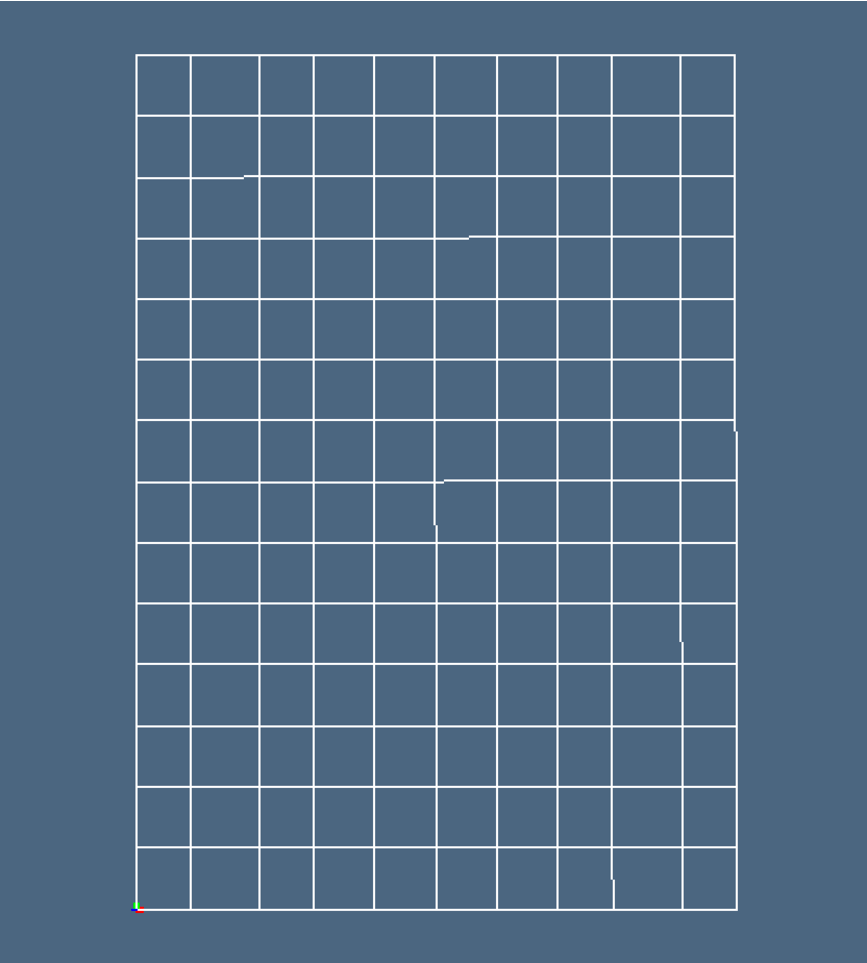
\includegraphics[width=0.33\linewidth]{images/hospitalgrid} 
   \caption{The reference grid used in the model construction. The intersections of grid lines have integer coordinates.}
   \label{fig:referencegrid2}
\end{figure}



\paragraph{From grid to metric coordinates}
The actual transformation of vertices of geometric data is executed by applying the (partial) function \texttt{metric} to a list of 2D points, as shown by the example below.

%-------------------------------------------------------------------------------
@D From grid to metric coordinates
@{""" From grid to metric coordinates """
def grid2coords(X,Y):
    xMeasures = list(cumsum(X))
    yMeasures = list(cumsum(Y))
    def grid2coords0(point):
        x,y = point[0:2]
        xint,yint = int(x), int(y)
        xdec,ydec = float(x-xint), float(y-yint)
        xcoord = xMeasures[xint] + xdec*X[xint+1]
        ycoord = yMeasures[yint] + ydec*Y[yint+1]
        if len(point)==2: return [xcoord, ycoord]
        else: return [xcoord, ycoord, point[2]]
    return grid2coords0

def coordMaps(YMAX):
    def coordMaps0(polyline):
        polyline = AA(grid2coords(X,Y))(polyline)
        polyline = vmap(YMAX)(polyline)
        return [eval(vcode(point)) for point in polyline]
    return coordMaps0

metric = coordMaps(YMAX)
@}
%-------------------------------------------------------------------------------


\paragraph{Example} 
A simple example of transformation from grid to metric coordinates is given here:
{\small 
\begin{verbatim}
polyline = metric([[3,4],[3,8],[4,8],[4,7.8],[6,7.8],[6,8],[6.65,8],[6.65,4]])
>>> [[24.5,84.0],[24.5,50.4],[32.9,50.4],[32.9,52.08],[49.7,52.08],[49.7,50.4],
     [55.16,50.4],[55.16,84.0]]
\end{verbatim}}

\paragraph{Mapping the grid frame to a Cartesian right-hand frame}
%-------------------------------------------------------------------------------
@D Mapping a grid frame to a Cartesian one
@{""" Mapping the grid frame to a Cartesian right-hand frame """
def vmap(YMAX):
    def vmap0(V):
        if len(V[0])==3: W = [[x,YMAX-y,z] for x,y,z in V]
        else: W = [[x,YMAX-y] for x,y in V]
        return W
    return vmap0
                
def embed(z):
    def embed0(p): 
        return p+[z]
    return embed0
@}
%-------------------------------------------------------------------------------


\paragraph{From array indices to grid coordinates}

The reference grid, as the Cartesian product of two subsets of adjacent integers, will be used both to strongly simplify the input of data, and to assign to such coordinate numbers a more interesting meaning. For example the open space in the middle of the building will so defined as the 2D box with extreme points of integer coordinates $(3,4)$ and $(7,11)$.
Therefore the whole building  will be contained in the 2D interval $[0,10]\times [0,14]$ in ``\emph{grid coordinates}''.

%-------------------------------------------------------------------------------
@D From array indices to grid coordinates
@{""" From array indices to grid coordinates """
def index2coords(theArray):
    return CONS(AA(T([1,2]))(CAT((theArray).tolist())))
@}
%-------------------------------------------------------------------------------


\bibliographystyle{amsalpha}
\bibliography{test}

\end{document}
